%! Author = kevin
%! Date = 2022-01-12


\usepackage{blindtext}
% Preamble
\documentclass[10pt]{article}
\title{Protein-Liganden-Docking\\\large{Bioinformatik gegen Malaria \& Co.}}
\author{Kevin Kretz, German Esaulkov, Leander Schäfer}
\date{\today}

% Packages
\usepackage{graphicx}
\usepackage{wrapfig}
% \usepackage{scrartcl}
\usepackage{amsmath}
\usepackage{listings}
\usepackage{xcolor}
\usepackage[german]{babel}
% \usepackage[clean]{svg}
\usepackage{csvsimple}
\usepackage[a4paper, portrait, margin=2.5cm]{geometry}
\usepackage[hyphens]{url}
\PassOptionsToPackage{hyphens}{url}\usepackage{hyperref}
\usepackage{float}

% Code
\definecolor{codegreen}{rgb}{0,0.6,0}
\definecolor{codegray}{rgb}{0.5,0.5,0.5}
\definecolor{codepurple}{rgb}{0.58,0,0.82}
\definecolor{backcolour}{rgb}{0.95,0.95,0.92}

\lstdefinestyle{mystyle}{
    backgroundcolor=\color{backcolour},
    commentstyle=\color{codegreen},
    keywordstyle=\color{magenta},
    numberstyle=\tiny\color{codegray},
    stringstyle=\color{codepurple},
    basicstyle=\ttfamily\footnotesize,
    breakatwhitespace=false,
    breaklines=true,
    captionpos=b,
    keepspaces=true,
    numbers=left,
    numbersep=5pt,
    showspaces=false,
    showstringspaces=false,
    showtabs=false,
    tabsize=2
}

\hypersetup{
    colorlinks=false,
    linkcolor=blue,
    filecolor=magenta,
    urlcolor=cyan,
    pdftitle={Dokumentation},
    pdfpagemode=FullScreen,
}

\lstset{style=mystyle}

% Config
\graphicspath{ {media_in_doc/} }


% Document
\begin{document}

    %\csvreader[tabular=|c|c|c|c|c|c|c|c|,
    %    table head=\hline Index & MODEL & RMSD_LB & RMSD_UB & SCORE & SDFMoleculeName & kkSMILES & kkTORSDO\\\hline,
    %    late after line=\\\hline]%
    %{pf_table_sorted_01.csv}{Index=\kkIndex,MODEL=\kkModel,RMSD_LB=\kkRMSDLB,RMSD_UB=\kkRMSDUB,SCORE=\kkScore,
    %SDFMoleculeName=\kkSDFMoleculeName,SMILES=\kkSMILES,TORSDO=\kkTORSDO}%
    %{\thecsvrow, \}%
    % {\kkIndex & \kkModel & \kkRMSDLB & \kkRMSDUB & \kkScore & \kkSDFMoleculeName & \kkSMILES & \kkTORSDO}%

    % \csvautotabular{pf_table_sorted_01.csv}

    \maketitle

    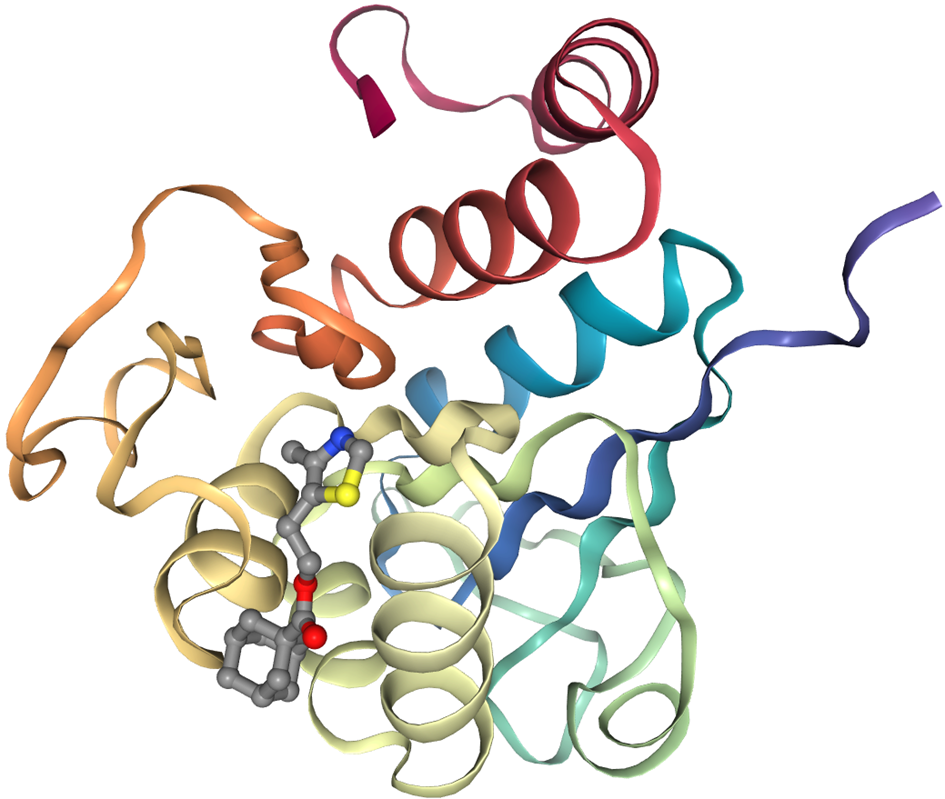
\includegraphics[width=\linewidth]{Titelbild}

    \pagebreak


    \section{Kurzfassung}\label{sec:kurzfassung}

    Tropenkrankheiten stellen in ihren Verbreitungsgebieten eine extreme Bedrohung für die dortige Bevölkerung dar.
    Gemessen an ihrer Bedeutung - Malaria ist z.B.\ mit 200 Millionen Fällen pro Jahr eine der häufigsten
    Infektionskrankheit der Welt - erhalten sie in nicht betroffenen Industrieländern nur wenig Aufmerksamkeit in den
    Medien, in Form von Forschungsprojekten und in den Entwicklungsabteilungen von Pharmafirmen.

    Aufgrund der Veröffentlichung des AlphaFold2-Papers im Juli 2021 und der gleichzeitig veröffentlichten Datenbank
    von dreidimensionalen Proteinmodellen sowie dem UseGalaxy-Server der Universität Freiburg haben wir gute
    Voraussetzungen bekommen, um mithilfe von Protein-Liganden-Docking nach möglichen Wirkstoffen gegen
    Tropenkrankheiten zu suchen.


    \section{Inhaltsverzeichnis}\label{sec:inhaltsverzeichnis}

    \tableofcontents

    \pagebreak


    \section{Einleitung}\label{sec:einleitung}

    Tropenkrankheiten richten in Entwicklungsländern verheerende Schäden an und fordern immer noch viele Opfer. So
    ist z.B.\ Malaria mit 200 Millionen Fällen pro Jahr eine der häufigsten Infektionskrankheit der Welt.
    Trotz der enormen Probleme, die Tropenkrankheiten wie z.B.\ Malaria, die Afrikanische Schlafkrankheit und die
    Chagas-Krankheit bereiten, schenken
    Industrieländer und die Pharmakonzerne diesen Bedrohungen nur wenig Beachtung.\cite{24} Die Entwicklung von
    Medikamenten gegen diese weit verbreiteten Krankheiten erscheint den Konzernen als nicht
    lukrativ genug, obwohl der Bedarf dafür vorhanden ist, und wird dementsprechend vernachlässigt.
    Doch mittlerweile gibt es Vereinigungen, die gegen diese reale Gefahr kämpfen.\cite{22}
    Wir möchten uns diesen, soweit es uns möglich ist, anschließen. Nun versuchen wir bei unserem Projekt mithilfe
    von Bioinformatik (weitere) helfende Wirkstoffe zu finden und unter Umständen auch eine neue Entdeckung zu machen.
    Selbstverständlich wird es uns nicht möglich sein, auf diese Weise ein fertiges Medikament entwickeln, dennoch
    hoffen wir, eine Grundlage für weitere Forschung schaffen zu können.

    \paragraph{Krankheiten}

    \begin{wrapfigure}{r}{0.3\textwidth}
        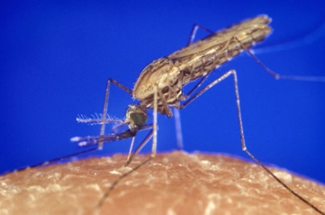
\includegraphics[width=\linewidth]{Anophelesmucke}
        \caption{Die Anophelesmücke beim Blutsaugen (CDC/James Gathany)}
    \end{wrapfigure}

    Doch warum haben wir ausgerechnet diese Krankheiten gewählt? Malaria, auch als Sumpf- oder Tropenfieber bekannt,
    ist die häufigste Tropenkrankheit. Sie ist vor allem in den tropischen Regionen Afrikas anzutreffen, aber auch in
    Südostasien und in den nördlichen Teilen Südamerikas. Der wichtigste Überträger der Krankheit ist die weibliche
    Anophelesmücke. Malaria kann Symptome wie Fieber, Erbrechen, Gelbsucht und Krämpfe hervorrufen. Vor allem die von
    uns gewählte Variante der Falciparum-Malaria ruft schwere Symptome wie Lähmung oder Koma hervor. Über Lungen-
    oder Nierenversagen führt die Krankheit zum Tod.

    \begin{wrapfigure}{r}{0.3\textwidth}
        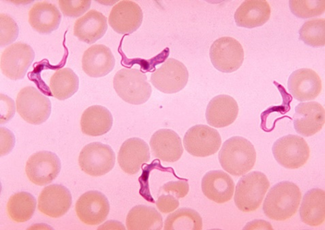
\includegraphics[width=\linewidth]{Trypanosoma}
        \caption{Trypanosoma, die Erreger der Schlafkrankheit (CDC/Dr. Myron G. Schultz)}
    \end{wrapfigure}

    Ebenfalls eine durch ein Insekt verbreitete Krankheit ist die \emph{Afrikanische Trypanosomiasis}, oder auch
    Afrikanische Schlafkrankheit, deren Erreger \emph{Trypanosoma brucei} durch die Tsetse-Fliege übertragen wird.
    Man kann
    aktuell mit ca. 500.000 Betroffenen in Afrika rechnen.\cite{25} Über Fieber, Gliederschmerzen,
    Lymphknotenschwellung und
    Anämie führt die Krankheit zum namengebenden Dämmerzustand und anschließend zum Tod.

    Als dritte Krankheit betrachten wir die Chagas-Krankheit, auch \emph{Südamerikanische Trypanosomiasis} genannt. Der
    Erreger \emph{Trypanosoma cruci}, ein Verwandter der \emph{Trypanosoma brucei}, wird durch den Kot verschiedener
    Raubwanzen,
    aber vor allem von \emph{Triatoma infestans}, übertragen.\cite{27} Aktuell gibt es ca. 18 Millionen Erkrankte,
    wobei
    jedes Jahr
    50.000 dazukommen. Die Zahl der Todesfälle beträgt jährlich um die 15.000. Die Krankheit verursacht Ödeme,
    chronisches Herzversagen und das Absterben von Nervenzellen im Darm. Dies führt teilweise zum Tod durch
    Darmverschluss oder Darmdurchbruch.

    Sowohl die Chagas-Krankheit als auch die \emph{Afrikanische Trypanosomiasis} sind von der
    Weltgesundheitsorganisation
    als \emph{Neglected Tropical Diseases} (NTD´s), also als \texttt{Vernachlässigte Tropenkrankheiten}, eingestuft. Die
    Auswirkungen dieser Vernachlässigung sind in den betroffenen Ländern deutlich zu spüren, weshalb also
    schnellstmöglich Mittel gegen diese Seuchen gefunden und entwickelt werden sollten.

    \paragraph{Verfahren}
    Wir möchten mithilfe von Protein-Liganden-Docking, einer Molecular Modelling-Technik, wobei mittels
    informatischer Methoden versucht wird, herauszufinden, wie Liganden mit Proteinen an welcher Stelle binden,
    Wirkstoffe für potenzielle Medikamente finden. Die Bindung eines Liganden an ein Protein kann die Struktur und
    die Funktion desselben beeinflussen bzw. verändern.\cite{23} Die Bindungsart ist eine chemische Bindung wie eine
    Ionenbindung, Wasserstoffbrückenbindung oder Van-der-Waals-Kräfte. Man benötigt dementsprechend Daten über den
    Liganden und den Rezeptor des Proteins.\cite{38}

    Dieses Verfahren hat eine große pharmazeutische Bedeutung, da man „in silico“ mögliche Moleküle finden kann, die
    vitale Proteine
    des Krankheitserregers außer Kraft setzen können, ohne dass alle Kandidaten im Labor untersucht werden müssen.
    Dadurch können sehr schnell sehr viele Wirkstoffkandidaten kostengünstig getestet werden.

    Auch wir möchten dieses bioinformatische Verfahren anwenden.

    \paragraph{Werkzeuge}
    Da wir persönlich keine Laborforschungsmittel oder Supercomputer besitzen, möchten wir öffentlich zugängliche
    Ressourcen verwenden.

    Dabei haben wir uns für die Galaxy-Plattform entschieden.

    \begin{wrapfigure}{r}{0.28\textwidth}
        
\includegraphics[width=\linewidth]{Galaxy-logo}
        \caption{Logo von Galaxy Europe}
    \end{wrapfigure}

    Galaxy ist eine browserbasierte Plattform für Computational Science, mit Fokus auf Biologie, die das Nutzen
    bioinformatischer Tools mit überschaubaren Programmierkenntnissen möglich macht. Die Abläufe werden
    zusammen mit den Daten in sogenannten \emph{Histories} gespeichert,
    die auch veröffentlicht werden können.\cite{17, 26}

    \begin{wrapfigure}{r}{0.28\textwidth}
        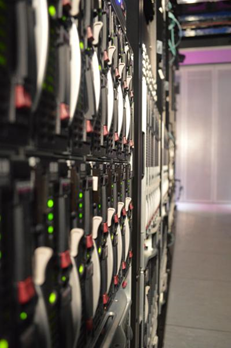
\includegraphics[width=\linewidth]{Datacenter}
        \caption{Datencenter des EMBL-EBI (EMBL-EBI)}
    \end{wrapfigure}

    Wir haben die öffentlich zugängliche, europäische Galaxy-Instanz (\url{https://usegalaxy.eu}) verwendet, da uns
    ihr großes Cluster genügend Rechenleistung für unser Projekt zur Verfügung stellt.
    Sie wird maßgeblich an der Uni Freiburg entwickelt und betrieben.
    Dort wollen wir, Protein-Liganden-Docking zu simulieren und auf diese
    Weise wirkungsvolle Moleküle gegen die Krankheiten zu finden.

    Mit Galaxy haben wir nun also schon eine gute Grundlage zur Erforschung und Durchführung des
    Protein-Liganden-Dockings, jedoch fehlen uns die Daten über den Wirkstoff, also den Liganden, und das Organell,
    sprich ein vitales Protein, welches im Erreger außer Kraft gesetzt werden soll, sodass er stirbt. Man benötigt
    also Datenbanken mit den entsprechenden Sequenzen bzw. Strukturen. Lange Zeit war das Bestimmen der räumlichen
    Struktur von Proteinen eins der großen Probleme in der Bioinformatik. Durch die von DeepMind entwickelte
    AlphaFold-Software und die daraus resultierenden Daten in der AlphaFold Protein Structure Database hat sich hier
    die Lage stark verbessert, was zu genaueren Docking-Vorhersagen führt. Die AlphaFold Protein Structure Database
    führt Proteinstrukturen auf, die von einer KI auf Grundlage der Aminosäurensequenz ermittelt bzw. vorhergesagt
    wurden.\cite{13} Dabei sind diese Vorhersagen sehr präzise.
    Hat man dann eine mögliche Struktur für das Protein gefunden,
    kann man nach realen Chemikalien in der EMBL-EBI-Datenbank, bzw. der von EMBL-EBI betriebenen Datenbank für
    bioaktive Moleküle ChEMBL suchen.\cite{7, 9, 10, 30} Das \emph{European Molecular Biology
    Laboratory Bioinformatics Institute}
    beherbergt
    die größte öffentlich zugängliche biologische Datenbank und bietet gleichzeitig auch bioinformatische Dienste für
    Forschende aus aller Welt an. Nur mithilfe von Galaxy, AlphaFold und EMBL-EBI bzw. ChEMBL können wir unser
    Projekt durchführen.

    Wie genau das abläuft wird im weiteren Verlauf erläutert.


    \section{Vorgehensweise, Materialien und Methode}\label{sec:vorgehensweise-materialien-und-methode}

    \subsection{Proteine und natürliche Liganden finden}\label{subsec:proteine-und-natuerliche-liganden-finden}

    Zunächst gilt es, Proteine zu finden, welche für wichtige Funktionen der Erreger verantwortlich sind.
    Hierzu betrieben wir Internetrecherchen, bei denen wir nach folgenden Kriterien geeignete Proteine auswählten:

    \begin{itemize}
        \item Die Struktur des Proteins im gefalteten Zustand ist bekannt, bzw. wird von AlphaFold mit großer
        Sicherheit vorhergesagt.
        \item Das Protein ist wichtig für die Lebensfähigkeit des Organismus.
        \item Der natürliche Ligand des Proteins ist bekannt.
        \item Das Protein ist nicht zu groß.
    \end{itemize}

%\subsubsection{Krankheiten wählen}\label{subsubsec:krankheiten-waehlen}

    \subsubsection{Malaria}\label{subsubsec:malaria}

    \paragraph{Protein}

    Unsere Forschung mit dem Malaria-Erreger \emph{Plasmodium Falciparum} baut auf einer im \emph{Malaria Journal}
    veröffentlichten Studie aus dem August des Jahres 2021 auf, in der man potenzielle Zielproteine für eine
    Behandlung von Malaria identifizierte.
    Wir wählten das Protein \emph{Protein DJ-1}
    (\texttt{C6KTB1\_PLAF7};
    UniProt: \texttt{C6KTB1}), da es ein kleines Protein ist, für welches
    AlphaFold eine sehr genaue Strukturvorhersage liefert.\cite{1}
    Wir mussten dann auf AlphaFold nur die UniProt-ID eingeben und konnten die PDB-Datei der Modellierung des
    Proteins herunterladen.

    \paragraph{Ligand}
    Nun suchten wir den natürlichen Liganden des Proteins.
    Nach einer Weile fanden wir in der ChEBI-Moleküldatenbank
    ein Molekül namens \texttt{5-(2-hydroxyethyl)-4-methylthiazole} mit der ChEBI-ID \texttt{17957}.\cite{11}
    Auf der Seite war eine MOL-Datei verfügbar.
    Wie wir zum SMILES-String gelangten, wird später beschrieben.

    \subsubsection{Afrikanische Schlafkrankheit}\label{subsubsec:afrikanische-schlafkrankheit}

    \paragraph{Protein}
    Dieser Organismus verfügt über das Hitzeschockprotein 83, das die Reifung, den Strukturerhalt und die
    ordnungsgemäße Regulierung spezifischer Zielproteine fördert, die z.B.\ an der Kontrolle des Zellzyklus und der
    Signaltransduktion beteiligt sind.

    \paragraph{Ligand}
    Durch Recherche im Internet fanden wir heraus, dass der natürliche Ligand des HSP83 folgender
    ist: \texttt{CHEMBL561224}. Auf seinem ChEMBL-Eintrag stand sein PDBe-Eintrag verlinkt (PDBe steht für Protein
    Data Bank
    in Europe). Von dort kamen wir auf den betreffenden PDBeChem-Eintrag, wo der SMILES-String \texttt{FC(F)(F)c2nn
        (c1c2C
        (=O)CC(C1)(C)C)c4ccc(C(=O)N)c(NC3CCC(O)CC3)c4} anzutreffen war.

    \subsubsection{Chagas-Krankheit}\label{subsubsec:chagas-krankheit}

    \paragraph{Protein}
    Im Fall der Chagas-Krankheit entschieden wir uns, einen etwas anderen Ansatz zu verfolgen. Wie auch die Afrikanische
    Schlafkrankheit, wird die Chagas-Krankheit durch einen Flagellaten aus der Gattung der Trypanosomen
    verursacht, genauer durch \emph{Trypanosoma bruci}.\cite{5} Trypanosomen nutzen Ergosterin statt Cholesterin
    als Baustein
    ihrer
    Zellmembranen.\cite{31} Die Blockierung der Ergosterin-Biosynthese stellt also eine mögliche Behandlung von
    Trypanosomen-Erkrankungen dar. Also wollten wir das Ergosterin angreifen, es binden. Als zu bindendes Protein
    wählten wir \emph{Sterol 14-alpha demethylase} (UniProt-ID \texttt{Q7Z1V1}) aus, das zur Biosynsthese von
    Ergosterol bei
    \emph{Trypanosoma cruzi} notwendig ist.

    \paragraph{Ligand}
    Um passende Liganden zu finden, gingen wir auf den Wikipedia-Artikel von Ergosterol und von dort aus auf die
    aufgelisteten Artikel der Inhibitoren (Azole). Diese waren \emph{Fluconazol}, \emph{Miconazol},
    \emph{Itraconazol}, \emph{Clotrimazol},
    \emph{Myclobutanil} und \emph{Lanosterol}.\cite{32, 33, 34, 35, 37} Von ihnen
    kopierten wir die SMILES-Strings, erstellten eine Compound
    library und
    fuhren wie gehabt fort.

    \subsection{Docking mit Galaxy}\label{subsec:galaxy}

    \subsubsection{Protein- und Ligandenstruktur eingeben}\label{subsubsec:protein--und-ligandenstruktur-eingeben}

    \begin{wrapfigure}{r}{0.5\textwidth}
        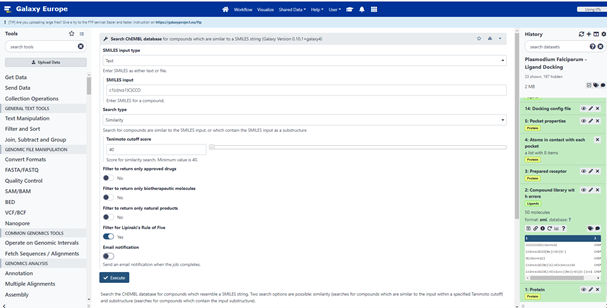
\includegraphics[width=\linewidth]{Aussehen der Galaxy-Website}
        \caption{GUI von Galaxy Europe}
    \end{wrapfigure}

    Auf der Galaxy-Website kann man eine neue Datenanalyse in Form einer sogenannten History erstellen.
    Darin stehen über das Web-Interface Tools zur Verfügung, die man nacheinander ausführen kann.
    Es handelt sich um graphisches Programmieren, wobei auch die Daten direkt in der History gespeichert sind.
    Histories können veröffentlicht oder geteilt werden.
    Als Leitfaden haben wir das Tutorial \emph{Protein-ligand-docking} verwendet.\cite{4}

    Nachdem eine History erstellt war, luden wir in der History als erstes über den \texttt{Upload-Data}-Button die PDB
    -Datei von \emph{Protein DJ-1} von unserem lokalen PC hoch.

    Dann brauchten wir eine Compound library, in welcher Moleküle aufgelistet sein sollten, die dem Molekül des
    natürlichen Liganden vom \emph{Protein DJ-1} ähnelten. Diese erstellten wir, indem wir das auf Galaxy
    bereitstehende Tool \texttt{Search ChEMBL database} nutzten.\cite{2} Dieses Tool ermöglicht es, die
    ChEMBL-Datenbank
    mithilfe
    des Tanimoto-Algorithmus nach Molekülen zu durchsuchen, die ähnlich zu einem Molekül sind, das man über einen
    einzugebenden SMILES-String übermittelt. Wir gaben also den SMILES-String \texttt{(c1(c(ncs1)C)CCO)} des natürlichen
    Liganden \texttt{(5-(2-hydroxyethyl)-4-methylthiazole)} als SMILES-Input ein. Diesen bekamen wir, indem wir die
    Mol-Datei
    von \emph{(5-(2-hydroxyethyl)-4-methylthiazole} in einer Galaxy-History hochluden und mit Compound conversion, einem
    auf Open Babel basierenden Dateiformat-Konvertierungstool, in eine SMILES-Datei umwandelten.\cite{3}

    \begin{wrapfigure}{r}{0.7\textwidth}
        \begin{subfigure}
            \includegraphics[width=0.3\linewidth]{Strukturformel natürlicher Ligand}
            \caption{Strukturformel natürlicher Ligand}
            \label{fig:nat-lig}
        \end{subfigure}
        \begin{subfigure}
            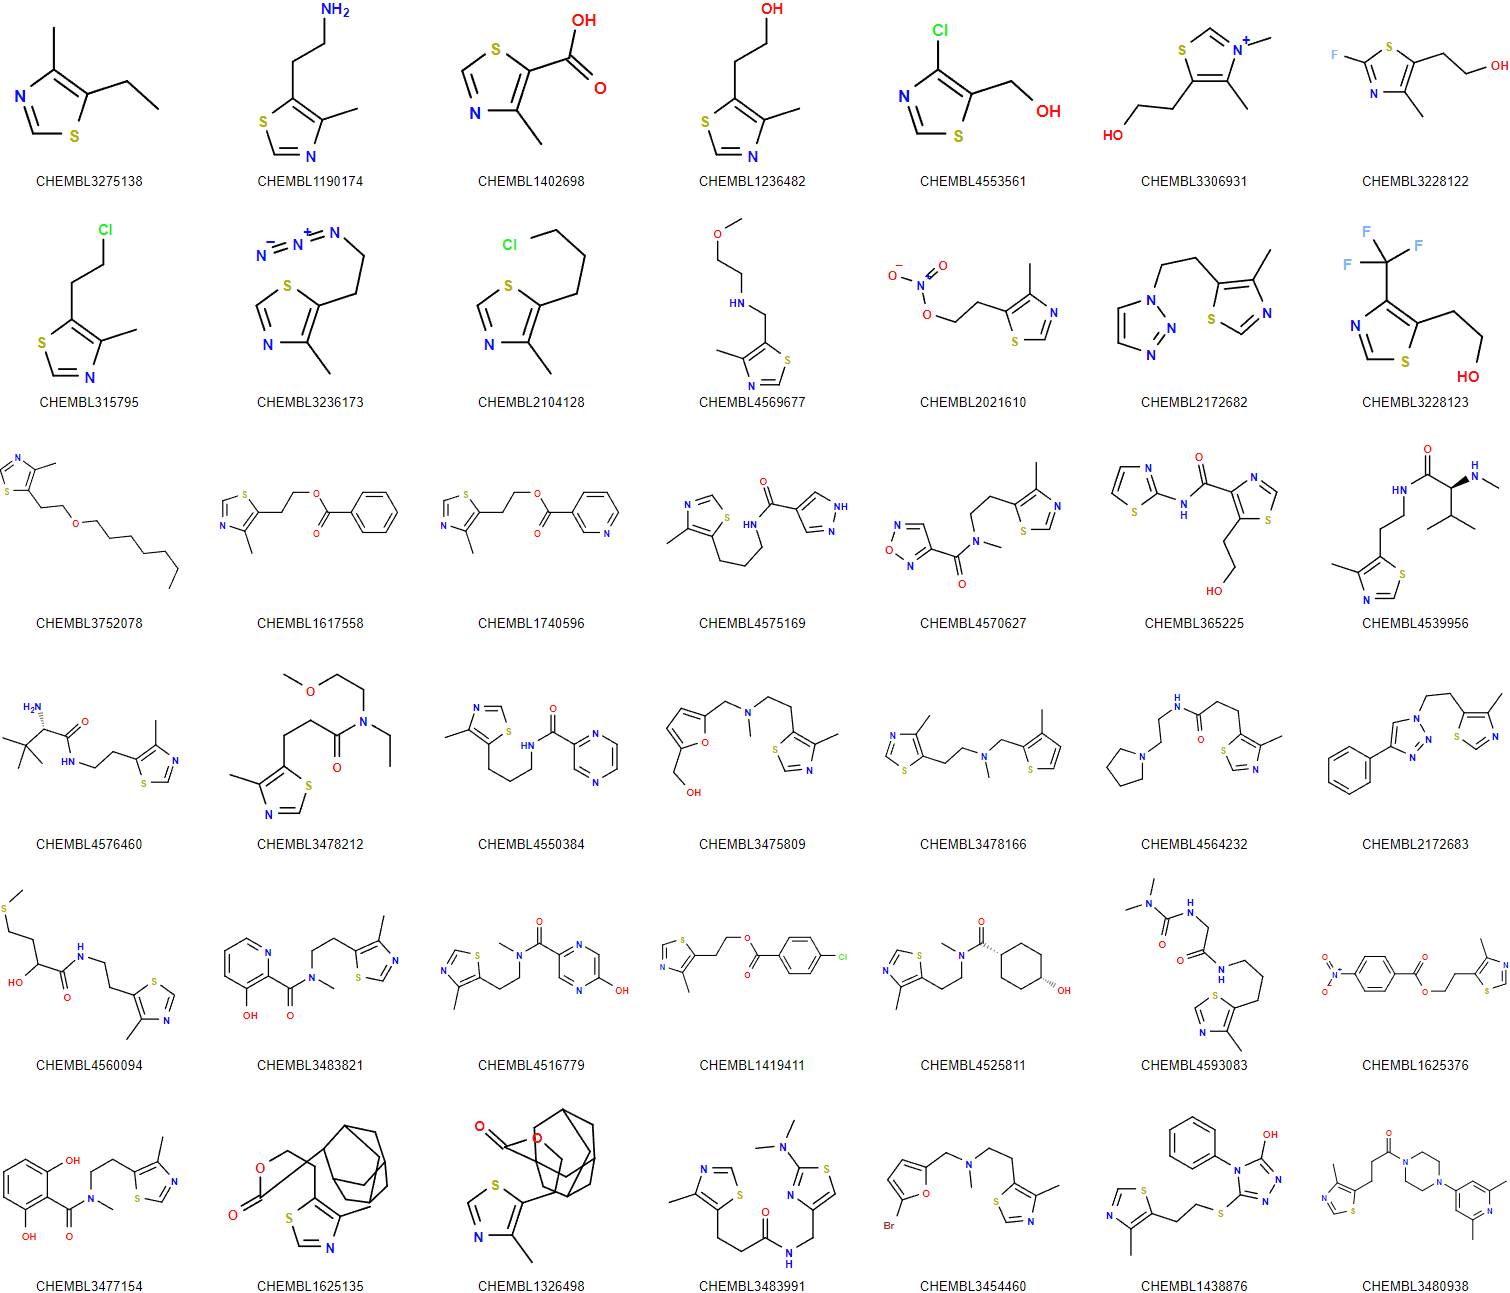
\includegraphics[width=\linewidth]{Strukturformeln Compound library}
            \caption{Strukturformeln Compound library}
            \label{fig:comp-lib}
        \end{subfigure}
        \label{fig:image2}
    \end{wrapfigure}

    In dem Tool konnte man auswählen, wie hoch der \emph{Tanimoto cutoff score} sein soll. Dieser Score entscheidet, wie
    hoch die Ähnlichkeit zwischen einem Liganden aus der Datenbank und dem eingegeben Vergleichsliganden sein muss,
    um in die Compound library aufgenommen zu werden. Ein Bereich von 40\% (niedrige Ähnlichkeit ist ausreichend) bis
    100\% steht zur Verfügung. Wir wählten 40\%. Außerdem haben wir ausgewählt, dass der \emph{Filter for Lipinski‘s
    Rule
    of Five} angewendet werden soll. Die Rule of Five ist eine Faustregel, die Moleküle auf ihre orale
    Bioverfügbarkeit überprüft, also auf die Frage, ob ein Molekül prinzipiell als oral einzunehmendes Arzneimittel
    geeignet wäre.\cite{28}

    Nach dem Ausführen dieses Befehls hatten wir nun also eine Compound library im Format einer SMILES-Liste, die aus
    50 Molekülen bestand, die dem natürlichen Liganden des \emph{Protein DJ-1} ähnlich sind, also auch
    prinzipiell
    stabile Bindungen erzielen sollten, und außerdem als Medikamente geeignet wären. Die Datei sieht folgendermaßen
    aus: In jeder Zeile ist ein Molekül aufgelistet, in der ersten Spalte steht der SMILES-String, in der zweiten der
    Titel, also die ChEMBL-ID des jeweiligen Moleküls.

    Die Abbildungen zeigen die Strukturformeln der Compound library und des natürlichen Liganden. Alle Moleküle aus der
    Compound library haben als Titel ihre ChEMBL-ID. Ähnlichkeiten sind zum Teil klar erkennbar.

    \subsubsection{Dateien für das Docking vorbereiten}\label{subsubsec:dateien-fuer-das-docking-vorbereiten}

    Nun konvertierten wir das Protein, also den Rezeptor, in eine PDBQT-Datei (wir nannten sie \emph{Prepared
    receptor}),
    die für das Docking benötigt wurde.

    Dann nutzten wir das \texttt{fpocket}-Tool, um überhaupt die Stelle auszumachen, an der der Ligand an das Protein
    docken
    sollte.\cite{16} Fpocket ist die wohl beste Möglichkeit, Bindungsstellen für kleine Moleküle zu ermitteln. Es
    ist ein
    Open-Source-Programm, welches mithilfe der Alpha-Sphären-Theorie arbeitet. Input war die PDB-Datei des Proteins,
    Output war zum einen eine Datei namens \texttt{Pocket properties}, in der die verschiedenen Eigenschaften der
    Taschen
    aufgelistet waren. Am wichtigsten war ihr Gesamtscore, nach dem wurden sie auch sortiert. Pocket1 war mit einem
    Score von rund 0,4 die beste.

    Zum anderen kam eine Dateiliste heraus, die alle acht Taschen im PDB-Format umfasste, also die Atome in Kontakt mit
    jeder Tasche.

    Danach konnten wir mit dem Tool \texttt{Calculate the box parameters using RDKit} eine Konfigurationsdatei für
    das Docking
    erstellen, die als Input pocket1 hatte und unter anderem die Größe des für das Docking benötigten Bereichs
    beinhaltet, also x-, y- und z-Puffer.\cite{15} Das Tool nutzt RDKit, eine Sammlung an Programmen für
    Chemieinformatik und
    maschinelles Lernen.\cite{14} Die Datei hieß \texttt{Docking config file}.

    Daraufhin mussten wir nur noch die Compound library mit dem Tool \texttt{Compound conversion} in eine SDF-Datei
    namens
    \texttt{Prepared ligands with errors} (Weshalb „with errors“, wird später erklärt.) umwandeln, und das Docking
    konnte
    beginnen.

    \subsubsection{Docking}\label{subsubsec:docking}

    Als Docking-Programm verwendeten wir AutoDock Vina, welches bei Galaxy über das Tool \texttt{Vina Docking} zur
    Verfügung
    steht.\cite{20, 21} AutoDock Vina ist ein Open-Source-Programm, das von \texttt{The Scripps Research
    Institute} entwickelt
    wurde.\cite{29} In
    Tests, in denen es mit anderen Molecular-Docking-
    Simulationsprogrammen verglichen wurde, schnitt es gut bis sehr
    gut ab und findet dementsprechend die größte Verwendung.

    AutoDock Vina legt um die pocket ein virtuelles dreidimensionales Gitter mit sehr kleinen Abständen im
    Angström-Bereich zwischen den einzelnen Gitterzeilen. An jeder Gitterkreuzung berechnet AutoDock für verschiedene
    räumliche Orientierungen einen Score, also pro Punkt und Orientierung (Pose). Bei der Scoring-Funktion werden
    sowohl intramolekulare als auch intermolekulare Bindungs- und Abstoßungskräfte bewertet. Auf diese Weise kann man
    am Ende die beste Pose eines Liganden zu einer pocket finden.

    Als Input verwendeten wir für den Rezeptor die PDBQT-Datei \texttt{Prepared receptor}, für die Liganden die
    SDF-Datei
    \texttt{Prepared ligands with errors} und als Box-Konfiguration die TXT-Datei \texttt{Docking config file}. Den
    pH-Wert setzten
    wir auf 7.4, den pH-Wert von menschlichem Blut.

    Das Ergebnis, eine SDF-Dateiliste, war jedoch als Fehler markiert, da acht der 50 SMILES-Strings nicht kompatibel
    waren. In der Fehlermeldung sahen wir nach, welche Liganden Probleme machten. Dort waren sieben Liganden
    aufgelistet, ein weiterer Ligand wurde zwar nicht in der Fehlermeldung aufgeführt, wurde jedoch auch nicht
    ausgeführt und war dementsprechend auch nicht nutzbar. Wir luden uns daraufhin die Compound library auf unseren
    PC herunter, öffneten sie mit einem Editor und löschten alle Problem-Liganden (es waren die Liganden Nummer 6, 9,
    12, 20, 27, 30, 39 und 45) manuell. Die Datei, die nun also noch 42 Liganden umfasste, luden wir wieder in der
    Galaxy-History unter dem Namen \texttt{Compound library without errors} hoch. Dort konvertierten wir sie wir
    gehabt in
    eine SDF-Datei und wiederholten das Docking mit denselben Inputs (selbstverständlich abgesehen von den Liganden).
    Nun war das Ergebnis eine funktionierende Dateiliste.

    \subsection{Auswertung der Daten}\label{subsubsec:aufbereitung-der-daten}

    \subsubsection{Compund library aufbereiten}

    \paragraph{Compound library-Erweiterung}
    Jetzt erstellten wir eine SMI-Datei des natürlichen Liganden, indem wir den schon am Anfang verwendeten
    SMI-String mit dem Titel \texttt{ligand} über den Button \texttt{Upload Data} und die Eingabemethode
    \texttt{Paste/Fetch data} mit der
    Einstellung \texttt{Convert spaces to tabs} eingaben. Die Datei nannten wir \texttt{Natural ligand}.

    Dann nutzten wir das Tool \texttt{Concatenate datasets}, um die Datasets \texttt{Natural ligand} und
    \texttt{Compound library without
    errors} zu einer SMI-Datei mit 43 Liganden zusammenzuführen. Dieses Dataset nannten wir \texttt{Labelled compound
    library}.

    \paragraph{Fingerprints und Clustering}
    Mit dem Tool \texttt{Molecule to fingerprint} erstellten wir aus der Labelled compound library eine Open Babel FP2
    fingerprints-Datei.\cite{8, 18} Molekulare Fingerprints kodieren Molekülstrukturen in Bits. Mit ihnen
    kann man Moleküle auf
    ihre Ähnlichkeit untersuchen.

    Danach konnten wir mit der Fingerprints-Datei als Input die Liganden mit dem Tool \texttt{Taylor Butina
    clustering} in
    Cluster einsortieren.\cite{6} Der Taylor-Butina Algorithmus erstellt Cluster, in denen Moleküle aufgelistet
    sind, die zu
    dem zentralen Molekül des Clusters eine bestimmte Ähnlichkeit aufweisen. Den Ähnlichkeits-Schwellenwert kann man
    im Tool angeben, wir haben 0,8 verwendet. Das Taylor-Butina Clustering ist (im Gegensatz zum nächsten
    Clustertool, welches wir verwenden werden) nicht hierarchisch, es gibt also keine Über- und Untercluster.

    Dann erstellten wir noch mit dem Tool \texttt{NxN clustering} ein Cluster-Dendogramm. Jenes wurde erzeugt, indem das
    Tool eine Selbstähnlichkeitsmatrix erstellte, um die Ähnlichkeit zu ermitteln.

    \subsubsection{Ergebnisse des Dockings auswerten}

    \paragraph{Veranschaulichung}
    Um die Ergebnisse des Dockings, die bisher noch in unterschiedlichen SDF-Dateien lagen, übersichtlicher zu
    machen, verwendeten wir das Tool \texttt{Extract values from an SD-file}. Input war die im Docking-Schritt erstellte
    Liste aus SDF-Dateien, Output eine Liste aus Tabular-Dateien, die die Informationen anders, übersichtlicher,
    darstellten.

    Nun wäre \emph{eine} Datei mit allen Ergebnissen praktisch. Um dies zu realisieren kam das Tool \texttt{Collapse
    Collection}
    zum Einsatz. Dieses reihte alle vom gerade benutzen Tool erstellten Dateien in einer Tabular-Datei hintereinander
    auf. Diese Datei sortierten wir mit dem Tool \texttt{Sort Dataset} nach dem Docking-Score.

    Dann hatten wir eine übersichtliche Datei, in der alle Ergebnisse des Dockings, also für jeden Liganden jede
    Torsion einzeln, nach Bindungsstabilität sortiert waren.

    Von den fünf Liganden, die die stabilsten Bindungen erzielt hatten, konvertierten wir danach noch die SDF-Dateien
    des Dockings mit \texttt{Compound conversion} in PDB-Dateien, um mit dem NGL-Viewer 3D-Visualisierungen von ihnen
    vornehmen zu können, das ist direkt in Galaxy möglich.\cite{19}

    Auf der Website von NGL konnten wir auch direkt die PDB-Datei des Proteins und die gerade erstellte PDB-Datei des
    Liganden hochladen, und so beide in der beim Docking bewerteten Position visualisiert betrachten.

    \paragraph{Substrukturen-Abgleich mit Python}
    Nun wollten wir ChEMBL nach Molekülen durchsuchen, die Moleküle aus unserer \texttt{Compound library without errors}
    als Substrukturen besitzen und die bereits als Medikament verwendet werden oder sich im Prozess der
    Medikamentenentwicklung befinden.
    Da ein solcher Abgleich manuell enorm Zeitintensiv gewesen wäre, automatisierten wir diesen mit Python.

    Das Repository ist unter \url{https://github.com/theKevinKretz/Protein-Ligand-Docking} auf
    GitHub veröffentlicht.

    Die ausführbare Datei ist
    die \href{https://github.com/theKevinKretz/Protein-Ligand-Docking/blob/master/main.py}{\texttt{main.py}}.

    Die Funktion \texttt{main()} ist die Hauptfunktion.
    Sie ruft für jede der SMI-Dateien im Inputverzeichnis \texttt{Input smi-files/} die Funktion
    \texttt{run\_for\_disease} auf.
    Die Funktion \texttt{run\_for\_disease} ruft wiederum die notwendigen Funktionen auf, um die jeweilige SMI-Datei
    zu bearbeiten.
    Hierzu wird für jeden SMILES-String in der SMI-Datei über die Funktion \texttt{substructure\_search()} eine
    Anfrage zu einer Substrukturen-Suche an die API der ChEMBL-Datenbank gesendet.
    Die Antwort des Servers wird durch die Funktion \texttt{store\_file()} gespeichert.
    Nun wird für jedes Ergebnis der Substrukturen-Suche der Wert \texttt{max\_phase} bestimmt.
    Wenn er größer als Null ist, werden die ChEMBL-ID des Originals aus der SMI-Datei, die des Ergebnisses der
    Substrukturen-Suche, sowie der \texttt{max\_phase}-Wert in der Dictionary-Variablen \texttt{everything} gespeichert.
    Der Inhalt der Variablen wird in der Datei \texttt{output.json} gespeichert und durch die Funktion
    \texttt{make\_look\_good} aufbereitet und in der Konsole ausgegeben.

    Von den gefundenen Ergebnissen suchten wir uns passende SMILES-Strings von Wikipedia, luden diese dann als
    SMI-Dateien hoch, präparierten sie für das Docking und dockten sie. Die Docking-Datei konvertierten wir wieder in
    eine Tabular-Datei. Danach konvertierten wir die SDF-Datei des gedockten Liganden in PDB-Dateien, erstellten aus
    der SMI-Datei des Medikamenten-Liganden und der bereits bestehenden \texttt{Labelled compound library} eine
    \texttt{Labelled compound library with drugs} und visualisierten deren Strukturformeln.

    Hier die Links zu den Malaria-Histories (SMILES-Vorbereitung und eigentliche History):

    \url{https://usegalaxy.eu/u/leander_schaefer/h/5-2-hydroxyethyl-4-methylthiazole-natural-ligand-of-protein-dj-1}

    \url{https://usegalaxy.eu/u/leander_schaefer/h/protein-dj-1---ligand-docking}

    % Abbildung 3: Flowchart Malaria

    \begin{figure}[H]
        \centering
        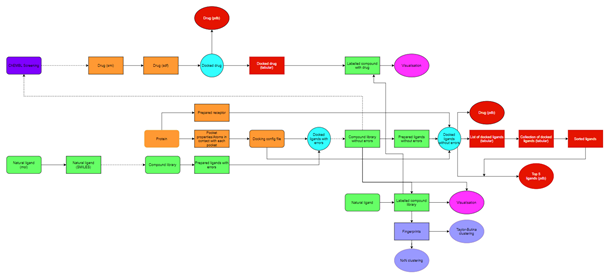
\includegraphics[width=0.7\linewidth]{malaria-flowchart}
        \caption{Flowchart: Malaria}
    \end{figure}

    \subsection{Andere Krankheiten}\label{subsubsec:andere-krankheiten}

    \subsubsection{Afrikanische Schlafkrankheit}
    Nach einem sehr ähnlichen Verfahren wie bei Malaria behandelten wir die Afrikanische Schlafkrankheit, genauer das
    für sie wichtige Hitzeschockprotein 83. Unterschiede lagen darin, dass das HSP 83 wesentlich mehr Taschen als
    das \emph{Protein DJ-1} von \emph{P. Falciparum} besaß (57). Außerdem umfasste die Compound library 52 Moleküle,
    welche von Anfang an alle
    funktionstüchtig waren, der bei Malaria notwendige Schritt des manuellen Löschens von Problem-Liganden, erneute
    Aufbereitung und erneutes Docking entfielen somit.

    Hier der Link zur Afrikanischen Schlafkrankheits-History:

    \url{https://usegalaxy.eu/u/leander_schaefer/h/hsp-83---ligand-docking-1}

    % Abbildung 4: Flowchart Afrikanische Schlafkrankheit

    \begin{figure}[H]
        \centering
        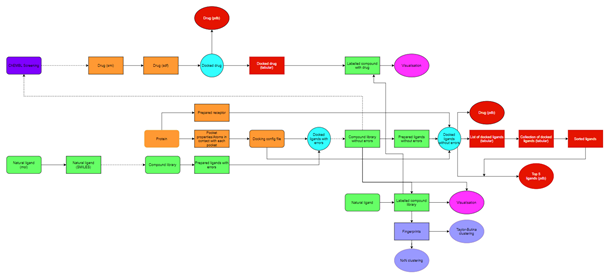
\includegraphics[width=0.7\linewidth]{afrikanische schlafkrankheit-flowchart}
        \caption{Flowchart: Afrikanische Schlafkrankheit}
    \end{figure}

    \subsubsection{Chagas-Krankheit}
    Auch bei der Chagas-Krankheit verwendeten wir, nachdem wir das Protein und die Compound library erstellt hatten,
    das bekannte Verfahren.
    Das Protein \emph{Sterol 14-alpha demethylase)} besitzt 37 pockets.

    Das Python-Script setzen wir hier nicht ein, da alle Liganden bereits als Medikamente in anderen
    Zusammenhängen eingesetzt werden.
    Uns ging es in diesem Fall einzig darum, herauszufinden, welche der
    Azolverbindungen am besten an die erst über Alphafold verfügbar gewordene Struktur des \emph{Trypanosoma
    cruzi}-Proteins passt.

    Hier der Link zur Chagas-History:

    \url{https://usegalaxy.eu/u/leander_schaefer/h/sterol-14-alpha-demethylase---ligand-docking-1}

    % Abbildung 5: Flowchart Chagas-Krankheit

    \begin{figure}[H]
        \centering
        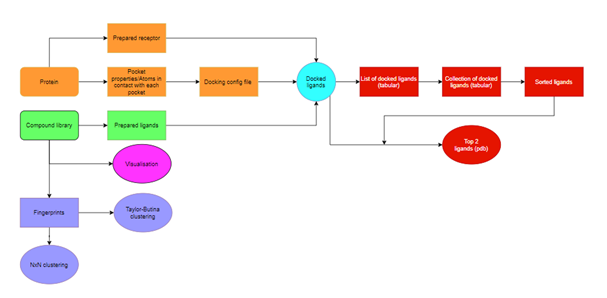
\includegraphics[width=0.7\linewidth]{chagas-flowchart}
        \caption{Flowchart: Chagas-Krankheit}
    \end{figure}


    \section{Ergebnisse}\label{sec:ergebnisse}

    \subsection{Malaria}\label{subsec:malaria}

    \subsubsection{Liganden-Clustering}

    \begin{wrapfigure}{r}{0.5\textwidth}
        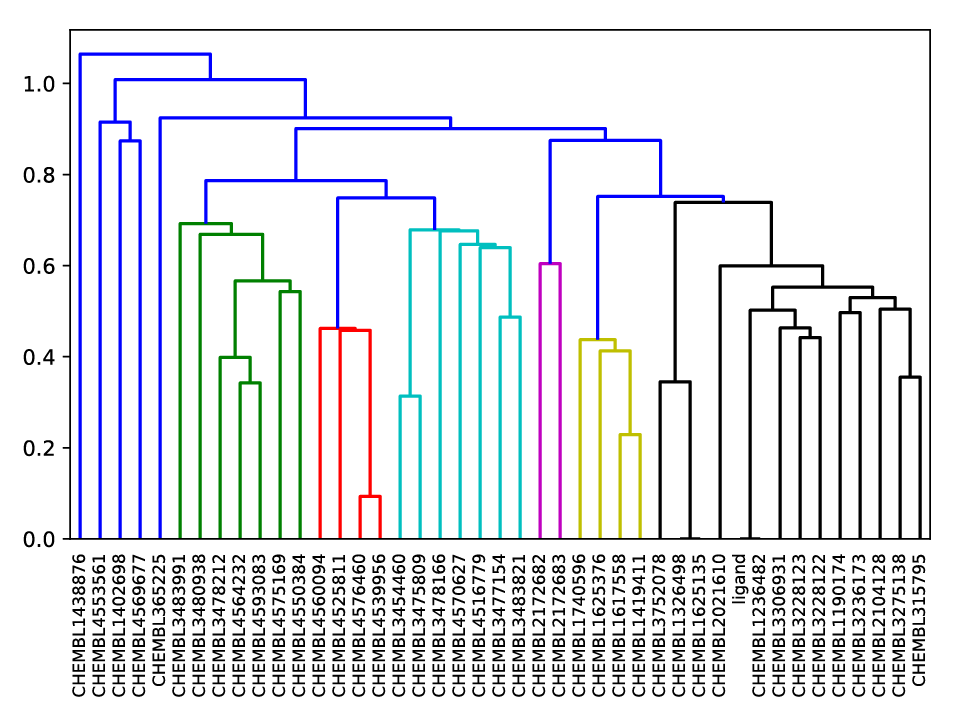
\includegraphics[width=\linewidth]{malaria-NxN_clustering}
        \caption{NxN-Clustering}\label{fig:nxn}
    \end{wrapfigure}

    Das Taylor-Butina Clustering ergab, dass im Fall von Malaria fünf Cluster bestehen.
    Der größte Cluster umfasste
    fünf Liganden, der zentrale Ligand war \texttt{CHEMBL3275138}, die „Cluster-Mitglieder“ waren
    \texttt{CHEMBL315795}, der natürliche
    Ligand, \texttt{CHEMBL1236482} und \texttt{CHEMBL1190174}.
    Des Weiteren existierten drei Cluster mit jeweils drei
    Liganden und ein kleiner, aus zwei Liganden bestehender Cluster.

    Das hierarchische Dendogramm des NxN-Clusterings sah folgendermaßen aus (\emph{ligand} ist nach wie vor der
    natürliche
    Ligand).

    % Abbildung 6: NxN-Clustering

    Je höher die Zahl auf der y-Achse, desto geringer ist die Ähnlichkeit. Die Ergebnisse sind denen des
    NxN-Clusterings ähnlich.

    \subsubsection{Docking-Ergebnisse}
    Dies ist die Tabular-Datei, die die Docking-Ergebnisse Torsion für Torsion, nach Score sortiert auflistet, hier
    die besten zehn Ergebnisse (SMILES-Strings aus Gründen der Übersichtlichkeit ausgenommen):

    \begin{center}
        \begin{tabular}{ c|c|c|c|c|c|c }
            Index & MODEL & RMSD\_LB & RMSD\_UB & SCORE & SDFMoleculeName & TORSDO \\
            \hline
            0     & 1.0   & 0.0      & 0.0      & -5.3  & CHEMBL1326498   & F 5    \\
            0     & 1.0   & 0.0      & 0.0      & -5.3  & CHEMBL1625135   & F 5    \\
            0     & 1.0   & 0.0      & 0.0      & -5.2  & CHEMBL3480938   & F 4    \\
            0     & 1.0   & 0.0      & 0.0      & -5.1  & CHEMBL2172683   & F 4    \\
            0     & 1.0   & 0.0      & 0.0      & -5.1  & CHEMBL3477154   & F 6    \\
            1     & 2.0   & 0.972    & 2.104    & -5.1  & CHEMBL1625135   & F 5    \\
            1     & 2.0   & 3.111    & 9.891    & -5.1  & CHEMBL3480938   & F 4    \\
            2     & 3.0   & 2.624    & 4.043    & -5.0  & CHEMBL3480938   & F 4    \\
            0     & 1.0   & 0.0      & 0.0      & -4.9  & CHEMBL1419411   & F 5    \\
            1     & 2.0   & 2.01     & 2.62     & -4.9  & CHEMBL1326498   & F 5
        \end{tabular}
    \end{center}


% 0 & 1.0 & 0.0 & 0.0 & -5.3 & CHEMBL1326498 & CC1=C(CCOC(=O)C23CC4CC(CC(C4)C2)C3)SC=N1 & F 5 \\
% 0 & 1.0 & 0.0 & 0.0 & -5.3 & CHEMBL1625135 & CC1=C(CCOC(=O)C2C3CC4CC(C3)CC2C4)SC=N1 & F 5 \\
% 0 & 1.0 & 0.0 & 0.0 & -5.2 & CHEMBL3480938 & CC1=CC(N2CCN(C(=O)CCC3=C(C)N=CS3)CC2)=CC(C)=N1 & F
% 0 & 1.0 & 0.0 & 0.0 & -5.1 & CHEMBL2172683 & CC1=C(CCN2C=C(C3=CC=CC=C3)N=N2)SC=N1 & F 4 \\
% 0 & 1.0 & 0.0 & 0.0 & -5.1 & CHEMBL3477154 & [H]OC1=CC=CC(O[H])=C1C(=O)N(C)CCC1=C(C)N=CS1 & F 6
% 1 & 2.0 & 0.972 & 2.104 & -5.1 & CHEMBL1625135 & CC1=C(CCOC(=O)C2C3CC4CC(C3)CC2C4)SC=N1 & F 5 \
% 1 & 2.0 & 3.111 & 9.891 & -5.1 & CHEMBL3480938 & CC1=CC(N2CCN(C(=O)CCC3=C(C)N=CS3)CC2)=CC(C)=N1
% 2 & 3.0 & 2.624 & 4.043 & -5.0 & CHEMBL3480938 & CC1=CC(N2CCN(C(=O)CCC3=C(C)N=CS3)CC2)=CC(C)=N1
% 0 & 1.0 & 0.0 & 0.0 & -4.9 & CHEMBL1419411 & CC1=C(CCOC(=O)C2=CC=C(Cl)C=C2)SC=N1 & F 5 \\
% 1 & 2.0 & 2.01 & 2.62 & -4.9 & CHEMBL1326498 & CC1=C(CCOC(=O)C23CC4CC(CC(C4)C2)C3)SC=N1 & F 5

    \begin{wrapfigure}{r}{0.2\textwidth}
        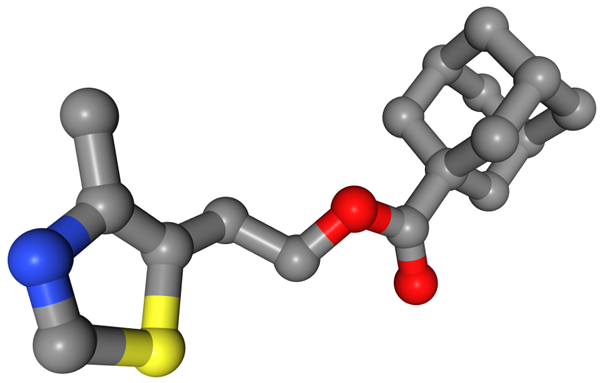
\includegraphics[width=\linewidth]{CHEMBL1326498}
        \caption{CHEMBL1326498}\label{fig:figure-CHEMBL1326498}
    \end{wrapfigure}

    Demnach sind die Liganden, die die fünf stabilsten Bindungen erzielt haben, die Liganden Nummer
    7: \texttt{CHEMBL1326498},
    38: \texttt{CHEMBL1625135}, 19: \texttt{CHEMBL3480938}, 36: \texttt{CHEMBL2172683} und 42: \texttt{CHEMBL3477154}.
    Dies ist eine NGL-3D-Visualisierungen von Ligand 7.

    % Abbildung 7: CHEMBL1326498


    Hier die Visualisierung von \texttt{CHEMBL1326498} und \emph{Protein DJ-1} in ihrer stabilsten Bindung:

    % Abbildung 8: P. Facliparum mit gedocktem CHEMBL1326498
    \begin{figure}[H]
        \centering
        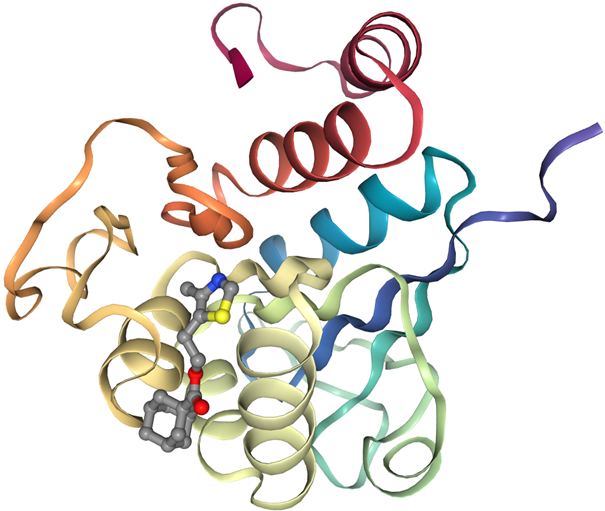
\includegraphics[width=0.6\linewidth]{Protein DJ-1 mit gedocktem CHEMBL1326498}
        \caption{Protein DJ-1 mit gedocktem CHEMBL1326498}\label{fig:figure-pf-CHEMBL1326498}
    \end{figure}

    Das Ergebnis des Python-Scripts bei Malaria war, dass ein Molekül aus unserer Compound library without errors,
    \texttt{CHEMBL315795} oder Colmethiazol unter dem Handelsnamen \emph{Heminevrin} bereits unter anderem gegen
    Schlafstörungen
    eingesetzt wird. Beim Docking hatte es mit einem Score von -2,7 aber bestenfalls ein Ergebnis im unteren Bereich.

    Der Ligand \texttt{CHEMBL1190174} aus unserer Compound library without errors ist ein Teil, also eine
    Substruktur, von
    \texttt{CHEMBL301265} (\emph{Pramipexole}), dass unter den Handelsnamen \emph{Mirapexin}, \emph{Neliprax},
    \emph{Oprymea} und \emph{Pipexus} schon
    unter anderem gegen Parkinson Verwendung findet.\cite{36} Das Ergebnis des Pramipexole-Dockings war, dass
    Pramipexole mit
    einem Score von -4,1 ziemlich gut bindet.

    % Abbildung 9: P. Facliparum mit gedocktem Pramipexole
    \begin{figure}[H]
        \centering
        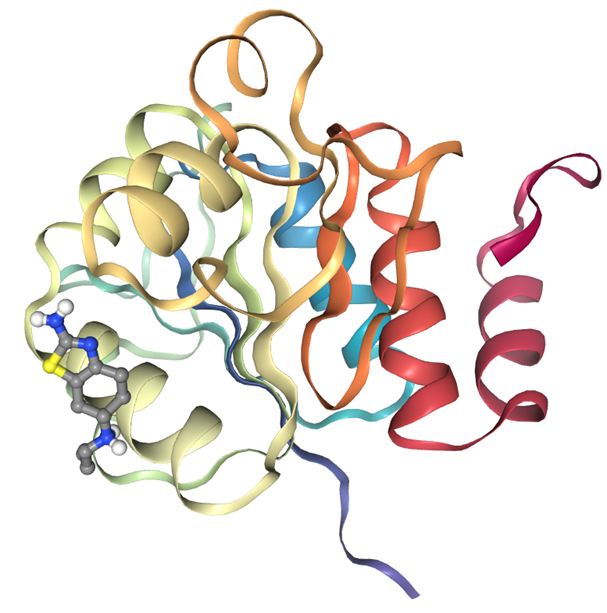
\includegraphics[width=0.6\linewidth]{Protein DJ-1 mit gedocktem Pramipexole}
        \caption{Protein DJ-1 mit gedocktem Pramipexole}\label{fig:figure-pf-pramipexole}
    \end{figure}

    \subsection{Afrikanische Schlafkrankheit}\label{subsec:afrikanische-schlafkrankheit}
    Bei der Afrikanischen Schlafkrankheit erreichten die Liganden 47: \texttt{CHEMBL561498} (Score: -11,1),
    52: \texttt{CHEMBL3235340}
    (Score: -10,9), 42: \texttt{CHEMBL407146} (Score: -10,5), 4: \texttt{CHEMBL259487} (Score: -10,4) und
    23: \texttt{CHEMBL3235351} (Score auch
    -10,4) die besten Bindungen mit dem Hitzeschockprotein 83.

    % Abbildung 10: HSP 83 mit gedocktem CHEMBL561498
    \begin{figure}[H]
        \centering
        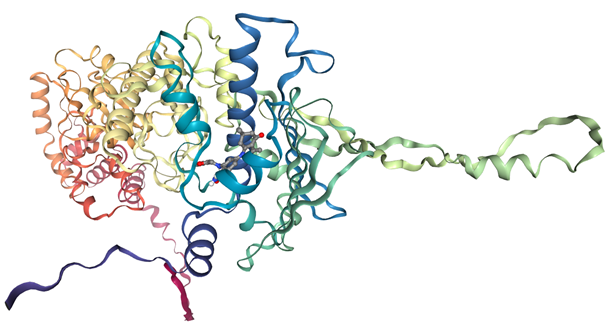
\includegraphics[width=0.6\linewidth]{HSP83 mit gedocktem CHEMBL561498}
        \caption{HSP83 mit gedocktem CHEMBL561498}\label{fig:figure-hsp-CHEMBL561498}
    \end{figure}

    Der Lauf des Python-Scripts ergab, dass viele Liganden aus der Compound library Substrukturen von
    \texttt{CHEMBL1195136}
    waren, welches sich in der Zulassungsphase 2 gegen Neoplasie bei Krebserkrankungen befindet. Den SMILES-String
    fanden wir auf der vom ChEMBL-Eintrag verlinkten J-Global-Eintrag zum betreffenden Molekül.\cite{12} Es dockte
    mit einem
    Score von -10,1 sehr gut.

    % Abbildung 11: HSP83 mit gedocktem CHEMBL1195136
    \begin{figure}[H]
        \centering
        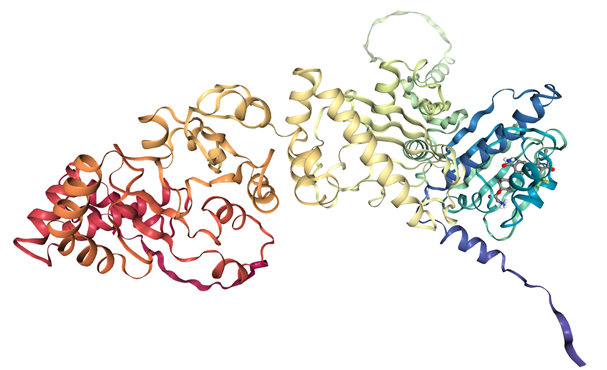
\includegraphics[width=0.6\linewidth]{HSP83 mit gedocktem CHEMBL1195136}
        \caption{HSP83 mit gedocktem CHEMBL1195136}\label{fig:figure-hsp-CHEMBL1195136}
    \end{figure}

    \subsection{Chagas-Krankheit}
    Bei der Chagas-Krankheit erreichte \emph{Itraconazol} mit einem Score von -9.8 einen ähnlich guten Wert für die
    Bindung
    an \emph{Sterol 14-alpha demethylase} wie deren natürlicher Ligand \emph{Lanosterol} (-9.7) und stellt damit den
    vielversprechendsten Inhibitor aus der von uns untersuchten Reihe von Azolverbindungen dar.

    % Abbildung 12: Sterol 14-alpha demethylase mit gedocktem Itraconazol
    \begin{figure}[H]
        \centering
        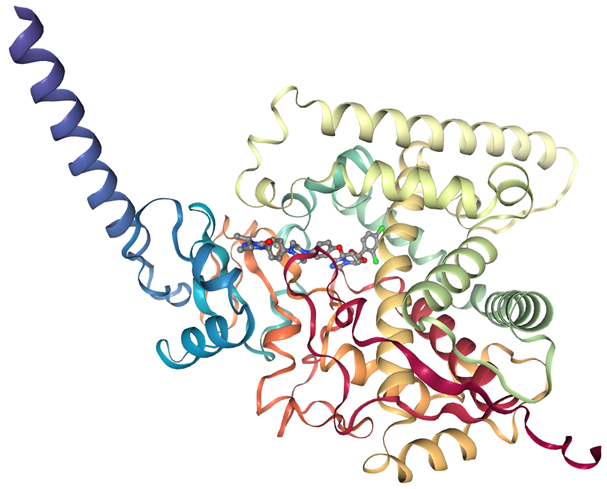
\includegraphics[width=0.6\linewidth]{Sterol 14-alpha demethylase mit gedocktem Itraconazol}
        \caption{Sterol 14-alpha demethylase mit gedocktem Itraconazol}\label{fig:figure-sterol-Itraconazol}
    \end{figure}


    \section{Ergebnisdiskussion}\label{sec:ergebnisdiskussion}
    Die Suche nach tatsächlich realistischen Liganden hat sich als komplizierter herausgestellt als anfangs erwartet.
    Erfreulicherweise konnten wir ein Python-Script schreiben, welches uns sehr bei der Arbeit geholfen hat. Dass wir
    damit auch bereits eingesetzte Arzneimittel gefunden haben, hat uns erstaunt und sehr gefreut.

    Mit den vorliegenden Wirkstoffen wäre im Prinzip die Grundlage für ein echtes Heilmittel schon geschaffen. Zur
    endgültigen Zulassung eines solchen fehlen aber natürlich noch die Tests im Labor und die klinischen Studien für
    die Wirksamkeit und Unbedenklichkeit bei der Anwendung.
    Wir haben leider nicht die Ressourcen für solche Studien,
    weshalb wir diese anderen Institutionen überlassen.
    Es ist aber dennoch bemerkenswert, welche Möglichkeiten
    allein die Verwendung öffentlicher Server, Datenbanken und frei verfügbarer Software im Bereich des
    Medikamenten-Screenings bieten.

    Wir hoffen mit unserer Arbeit die Aufmerksamkeit der Öffentlichkeit auf die Krankheiten und die betroffenen
    Länder zu ziehen und somit einen Beitrag für die Bekämpfung der Tropenkrankheiten zu leisten.


    \section{Zusammenfassung}\label{sec:zusammenfassung}
    Unsere Forschung mit Galaxy und Alphafold hat sich als ergebnisreich erwiesen und dabei haben sich viele
    Wirkstoffe als vielversprechend erwiesen: Zusammenfassend kann man sagen, dass es uns tatsächlich gelungen ist,
    Kandidaten für mögliche Medikamente gegen Malaria, die Afrikanische Schlafkrankheit und die Chagas-Krankheit zu
    finden.
    So könnte man nun beispielsweise Studien starten, um zu überprüfen, ob das Molekül \texttt{CHEMBL561498}
    tatsächlich als Medikament gegen die Afrikanische Schlafkrankheit wirkt.
    Noch aufwandsfreier, sowohl zeitlich als
    auch monetär, wäre es, Studien durchzuführen, in denen man testet, ob beispielsweise Itraconazol, welches bereits
    als Medikament eingesetzt wird, auch gegen die Chagas-Krankheit wirkt.


    \section{Quellen- und Literaturverzeichnis}\label{sec:quellen--und-literaturverzeichnis}

    \begin{thebibliography}{9}

\bibitem{1}
\url{https://malariajournal.biomedcentral.com/track/pdf/10.1186/s12936-021-03865-1.pdf} \emph{Ali, Fawad & Wali, Hira & Jan, Saadia & Zia, Asad & Aslam, Muneeba & Ahmad, Imtiaz & Afridi, Sahib & Khan, Asifullah. (2021). Analysing the essential proteins set of Plasmodium falciparum PF3D7 for novel drug targets identification against malaria. Malaria Journal. 10.1186/s12936-021-03865-1}
Abgerufen: 15.12.2021

\bibitem{2}
\url{https://jcheminf.biomedcentral.com/articles/10.1186/s13321-015-0069-3} \emph{Bajusz, D., Rácz, A. & Héberger, K. Why is Tanimoto index an appropriate choice for fingerprint-based similarity calculations?. J Cheminform 7, 20 (2015).}
Abgerufen: 08.01.2022

\bibitem{3}
\url{https://jcheminf.biomedcentral.com/articles/10.1186/1758-2946-3-33} \emph{Boyle, N. M., Banck, M., James, C. A., Morley, C., Vandermeersch, T., & Hutchison, G. R. (2011). Open Babel: An open chemical toolbox. Journal of Cheminformatics, 3(1).}
Abgerufen: 03.12.2021

\bibitem{4}
\url{https://training.galaxyproject.org/training-material/topics/computational-chemistry/tutorials/cheminformatics/tutorial.html} \emph{Simon Bray, 2021 Protein-ligand docking (Galaxy Training Materials).}
Abgerufen: 28.11.2021

\bibitem{5}
\url{https://journals.asm.org/doi/full/10.1128/AAC.42.12.3245} \emph{Frederick S. Buckner, Aaron J. Wilson, Theodore C. White, Wesley C. Van Voorhis, Induction of Resistance to Azole Drugs inTrypanosoma cruzi}
Abgerufen: ##########

\bibitem{6}
\url{https://pubs.acs.org/doi/10.1021/ci9803381} \emph{Butina, D. (1999). Unsupervised Data Base Clustering Based on Daylight\textquotesingles Fingerprint and Tanimoto Similarity: A Fast and Automated Way To Cluster Small and Large Data Sets. Journal of Chemical Information and Computer Sciences, 39(4), 747–750.}
Abgerufen: 28.12.2021

\bibitem{7}
\url{https://www.ebi.ac.uk/pdbe-srv/pdbechem/chemicalCompound/show/HIE} \emph{EMBL-EBI, HIE : Summary}
Abgerufen: 05.01.2021

\bibitem{8}
\url{https://jcheminf.biomedcentral.com/articles/10.1186/1758-2946-5-S1-P36} \emph{Dalke, A. (2013). The FPS fingerprint format and chemfp toolkit. Journal of Cheminformatics, 5(S1).}
Abgerufen: 28.12.2021

\bibitem{9}
\url{https://academic.oup.com/nar/article/43/W1/W612/2467881} \emph{Davies, M., Nowotka, M., Papadatos, G., Dedman, N., Gaulton, A., Atkinson, F., … Overington, J. P. (2015). ChEMBL web services: streamlining access to drug discovery data and utilities. Nucleic Acids Research, 43(W1), W612–W620.}
Abgerufen: 03.12.2021

\bibitem{10}
\url{https://www.ebi.ac.uk/chembl/} \emph{Gaulton A, Hersey A, Nowotka M, Bento AP, Chambers J, Mendez D, Mutowo P, Atkinson F, Bellis LJ, Cibrián-Uhalte E, Davies M, Dedman N, Karlsson A, Magariños MP, Overington JP, Papadatos G, Smit I, Leach AR. (2017) 'The ChEMBL database in 2017.' Nucleic Acids Res., 45(D1) D945-D954.}
Abgerufen: 07.12.2021

\bibitem{11}
\url{https://www.ebi.ac.uk/chebi/init.do} \emph{Hastings J, Owen G, Dekker A, Ennis M, Kale N, Muthukrishnan V, Turner S, Swainston N, Mendes P, Steinbeck C. (2016). ChEBI in 2016: Improved services and an expanding collection of metabolites. Nucleic Acids Res.}
Abgerufen: 07.12.2021

\bibitem{12}
\url{https://jglobal.jst.go.jp/en/detail?JGLOBAL_ID=201007072378971804#%7B%22category%22%3A%227%22%2C%22fields%22%3A%5B%7B%22op%22%3A%22AND%22%2C%22nm%22%3A%22SNID%22%2C%22vals%22%3A%5B%7B%22v%22%3A%22J2.821.849D%22%2C%22m%22%3A1%7D%5D%7D%5D%7D} \emph{J-Global, SNX-5422}
Abgerufen: 13.01.2022

\bibitem{13}
\url{https://alphafold.com} \emph{Jumper, J et al. Highly accurate protein structure prediction with AlphaFold. Nature (2021). Varadi, M et al. AlphaFold Protein Structure Database: massively expanding the structural coverage of protein-sequence space with high-accuracy models. Nucleic Acids Research (2021).}
Abgerufen: 03.12.2021

\bibitem{14}
\url{https://sourceforge.net/p/rdkit/wiki/Home/} \emph{Greg Landrum, RDKit Open-Source Cheminformatics and Machine Learning}
Abgerufen: 08.01.2022

\bibitem{15}
\url{http://www.rdkit.org/} \emph{Landrum, G. (n.d.). RDKit: Open-source cheminformatics.}
Abgerufen: 06.12.2021

\bibitem{16}
\url{https://bmcbioinformatics.biomedcentral.com/articles/10.1186/1471-2105-10-168} \emph{Le Guilloux, V., Schmidtke, P. & Tuffery, P. Fpocket: An open source platform for ligand pocket detection. BMC Bioinformatics 10, 168 (2009).}
Abgerufen: 05.12.2021

\bibitem{17}
\url{https://usegalaxy.eu/} \emph{The authors acknowledge the support of the Freiburg Galaxy Team: Dr. Wolfgang Maier and Björn Grüning, Bioinformatics, University of Freiburg (Germany) funded by the Collaborative Research Centre 992 Medical Epigenetics (DFG grant SFB 992/1 2012) and the German Federal Ministry of Education and Research BMBF grant 031 A538A de.NBI-RBC.}
Abgerufen: 27.11.2021

\bibitem{18}
\url{http://openbabel.org/docs/dev/Features/Fingerprints.html} \emph{Open Babel, Molecular fingerprints and similarity searching}
Abgerufen: 12.01.2022

\bibitem{19}
\url{http://nglviewer.org/ngl/} \emph{AS Rose, AR Bradley, Y Valasatava, JM Duarte, A Prlić and PW Rose. NGL viewer: web-based molecular graphics for large complexes. Bioinformatics: bty419, 2018.}
Abgerufen: 03.01.2022

\bibitem{20}
\url{https://vina.scripps.edu/} \emph{O. Trott, A. J. Olson, AutoDock Vina: improving the speed and accuracy of docking with a new scoring function, efficient optimization and multithreading, Journal of Computational Chemistry 31 (2010) 455-461}
Abgerufen: 03.12.2021

\bibitem{21}
\url{https://onlinelibrary.wiley.com/doi/10.1002/jcc.21334} \emph{Trott, O., & Olson, A. J. (2009). AutoDock Vina: Improving the speed and accuracy of docking with a new scoring function, efficient optimization, and multithreading. Journal of Computational Chemistry, NA-NA.}
Abgerufen: 03.12.2021

\bibitem{22}
\url{https://www.who.int/teams/control-of-neglected-tropical-diseases} \emph{World Health Organization, „Neglected tropical diseases“}
Abgerufen: 06.01.2022

\bibitem{23}
\url{https://en.wikipedia.org/wiki/Protein%E2%80%93ligand_docking} \emph{Wikipedia, Protein - Ligand Docking}
Abgerufen: 05.01.2022

\bibitem{24}
\url{https://de.wikipedia.org/wiki/Malaria#J%C3%A4hrliche_Opfer_und_Inzidenz} \emph{Wikipedia, Malaria}
Abgerufen: 05.01.2022

\bibitem{25}
\url{https://de.wikipedia.org/wiki/Afrikanische_Trypanosomiasis} \emph{Wikipedia, „Afrikanische Trypanosomiasis“}
Abgerufen: 06.01.2022

\bibitem{26}
\url{https://en.wikipedia.org/wiki/Galaxy_(computational_biology)} \emph{Wikipedia, Galaxy (computational biology)}
Abgerufen: 29.11.2021

\bibitem{27}
\url{https://de.wikipedia.org/wiki/Chagas-Krankheit} \emph{Wikipedia, Chagas-Krankheit}
Abgerufen: 06.01.2022

\bibitem{28}
\url{https://de.wikipedia.org/wiki/Rule_of_Five} \emph{Wikipedia, Rule of Five}
Abgerufen: 08.01.2022

\bibitem{29}
\url{https://en.wikipedia.org/wiki/AutoDock} \emph{Wikipedia, AutoDock}
Abgerufen: 08.01.2022

\bibitem{30}
\url{https://en.wikipedia.org/wiki/ChEMBL} \emph{Wikipedia, ChEMBL}
Abgerufen: 14.01.2022

\bibitem{31}
\url{https://en.wikipedia.org/wiki/Ergosterol} \emph{Wikipedia, Ergosterol}
Abgerufen: 09.01.2022

\bibitem{32}
\url{https://en.wikipedia.org/wiki/Fluconazole} \emph{Wikipedia, Fluconazole}
Abgerufen: 09.01.2022

\bibitem{33}
\url{https://en.wikipedia.org/wiki/Miconazole} \emph{Wikipedia, Miconazole}
Abgerufen: 09.01.2022

\bibitem{34}
\url{https://en.wikipedia.org/wiki/Clotrimazole} \emph{Wikipedia, Clotrimazole}
Abgerufen: 09.01.2022

\bibitem{35}
\url{https://en.wikipedia.org/wiki/Myclobutanil} \emph{Wikipedia, Myclobutanil}
Abgerufen: 09.01.2022

\bibitem{36}
\url{https://en.wikipedia.org/wiki/Pramipexole} \emph{Wikipedia, Pramipexole}
Abgerufen: 13.01.2022

\bibitem{37}
\url{https://en.wikipedia.org/wiki/Lanosterol} \emph{Wikipedia, Lanosterol}
Abgerufen: 09.01.2022

\bibitem{38}
\url{https://en.wikipedia.org/wiki/Ligand} \emph{Wikipedia, Ligand}
Abgerufen: 13.12.2021

\end{thebibliography}


    \section{Unterstützungsleistungen}\label{sec:unterstuetzungsleistungen}

    \begin{itemize}
        \item Herr Dr. Wolfgang Maier, Bioinformatiker, Technische Fakultät Freiburg: Generelle Unterstützung,
        Wissenschaftlicher Beirat, Korrekturlesen

        \item Lino Riepenhausen, Schüler: Korrekturlesen
    \end{itemize}

\end{document}

% todo unterst.
% todo inhaltsverz. doppelter titel